\chapter{Lösung}
\label{chap:loesung}
% In diesem Kapitel beschreiben Sie Ihre Lösung des Problems. Geben Sie dem Leser genügend Einblick in die Lösung, so dass er Ihre Arbeit entsprechend würdigen kann. Verwenden Sie aber Anhänge für Dinge, die hier nicht unbedingt bis ins letzte Detail verstanden werden müssen.
Aufgabenstellung: ``Ziel dieser Arbeit ist die Entwicklung und Anwendung eines Systems zur Speicherung (von Daten) in einer semantischen Datenbank$\cdots$''.~\cite{Aufgabenstellung} Kernpunkt: Verwendung einer semantischen Datenbank.

Semantik bedeutet einerseits Sammlung von neuen Theorien und neuen Technologien, andererseits beinhaltet sie eine zunächst ungewohnte Denkweise. Dies ist gerade für Personen aus der Informatik, speziell mit objektorientiertem Hintergrund eine Herausforderung. Die Erfahrungen und Schwierigkeiten der Autoren werden im~\autoref{sub:modellierung_der_ontologie} beschrieben.

Die Autoren stellten sich die  Anforderung, innerhalb einer bestimmten Wissensdomäne Fragen beantworten zu können (dies wurde bei der Auflistung der Meilensteine nicht erwähnt). Dies setzt bereits fundiertes Fachwissen der Thematik voraus, da Fragen anhand der Bedeutung der Inhalte (Semantik) beantwortet werden sollen.

Die Organisation sowie Vorgehensweise der Autoren wurden im \autoref{chap:administratives} und \autoref{chap:vorgehen} ausführlich beschrieben. Dieses Kapitel beschreibt die tatsächliche Lösung der Aufgabenstellung.

\section{Von der Wissenserarbeitung zum Tutorial}
\label{sec:loesung_tutorial}
Zunächst musste ein Tutorial erarbeitet werden, um die Theorien und Technologien zu bestimmen. Dabei war es schwierig, eine einfache, nutzbare Form zu erstellen und dabei dem Leser gleichzeitig genügend Hintergrundwissen zu vermitteln. Der Leser soll wirklich verstehen was Wissensmodellierung respektive ein Expertensystem bedeuten. Es entstand das Tutorialdokument, welches die Modellierung aus drei Perspektiven betrachtet. % TODO: Diese werden ausführlich im \autoref{subsec:dokumentation_wissensmodellierung_aufbau} beschrieben.

\section{Modellierung}
\label{sec:loesung_modellierung}
Semantische Datenbanken werden auf der Basis von Ontologien gebildet. Eine Ontologie wird für eine Problemdomäne erstellt und bildet deren Wissen ab. Problemdomäne dieser Arbeit ist das Reisen. Es wurde beschlossen sich auf Tages- und Wochenendausflüge in der Schweiz zu begrenzen. Die gesamte Modellierung wurde mit Hilfe von OWL formuliert. Bei OWL handelt es sich um eine Ontologieabbildungssprache. Benötigte Regeln werden in der Regelsprache SWRL ausgedrückt. Details dazu können im~\hyperref[sec:anhang:tutorial_dokument]{Tutorial} unter Kapitel 9 nachgelesen werden.

Um die Ontologie zu veranschaulichen, wurde diese grafisch in einem semantischen Netz abgebildet. Zur Vereinfachung wurde die Ontologie aufgeteilt und in entsprechenden semantischen Teilnetzen abgebildet. Sämtliche Grafiken finden sich als Anhang unter~\ref{chap:anh_modell_graph}.

Mit der Einschränkung der Problemdomäne konnten zwei Hauptklassen gebildet werden (Ausflüge und Restaurants).

Restaurant wie auch Ausflug werden durch Eigenschaften von Bedingungen (Bedingungs-Properties) beschrieben. Zum Beispiel könnte dabei ein Restaurantbesitzer die Qualität (Ambiente, Küche, Durchschnittspreise) seines Restaurants angeben.\\
Ausflüge werden durch zusätzliche Werte, wie der Anzahl Teilnehmer, den Öffnungszeiten des Ausflugzieles oder was ein Ausflug bietet oder erfordert beschrieben.

Mittels Regeln wurden die Folgerungen aus diesen Eigenschaften vordefiniert.

\begin{figure}[H]%[htbp]
    \begin{minipage}[hbt]{0,49\textwidth}
        \centering
        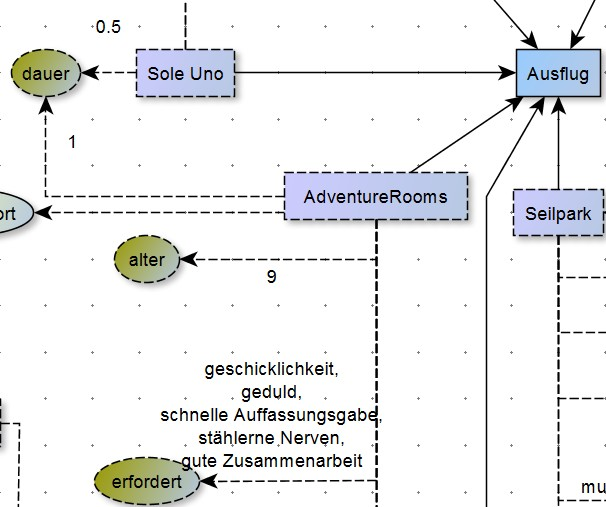
\includegraphics[scale=0.3]{bilder/charAusflug.jpg}
        \caption{Eigenschaften eines Ausflugs.\label{fig:charAusflug}\protect\footnotemark}
    \end{minipage}
    \begin{minipage}[hbt]{0,49\textwidth}
        \centering
        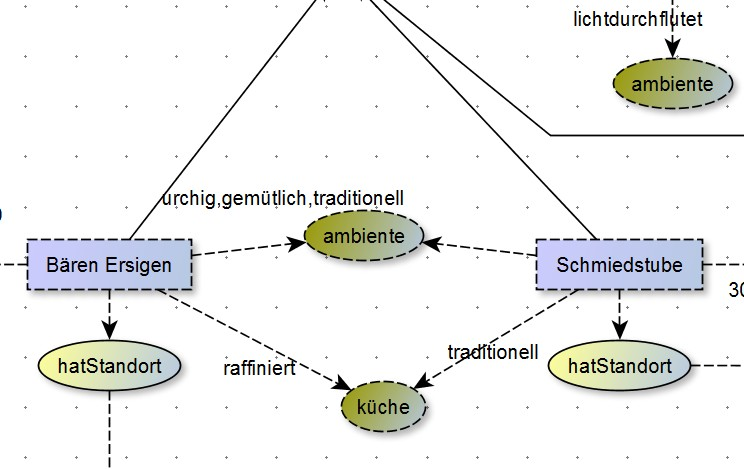
\includegraphics[scale=0.3]{bilder/charRestaurant.jpg}
        \caption{Eigenschaften eines Restaurants.\label{fig:charRest}\protect\footnotemark[1]}
    \end{minipage}
\end{figure}
\footnotetext{Eigene Darstellung mittels yEd.}


Um die verschiedenen Möglichkeiten beim Abbilden einer Ontologie aufzuzeigen, wurde für die Hauptklassen jeweils eine andere Umsetzung gewählt. Die Hauptklasse Restaurant hat verschiedene Unterklassen. Der Benutzer kann dadurch nach verschiedenen Arten von Restaurants suchen. Je nach gewählter Unterklassen (Art des Restaurants) müssen unterschiedliche Kriterien (Bedinungs-Properties) erfüllt sein. Die von den Autoren definierten Regeln lassen zum Beispiel auf ein Gourmetrestaurant schliessen, wenn dieses über eine raffinierte Küche (in Form von Bedingungsproperties) verfügt.

\begin{figure}[H]%[htbp]
    \centering
    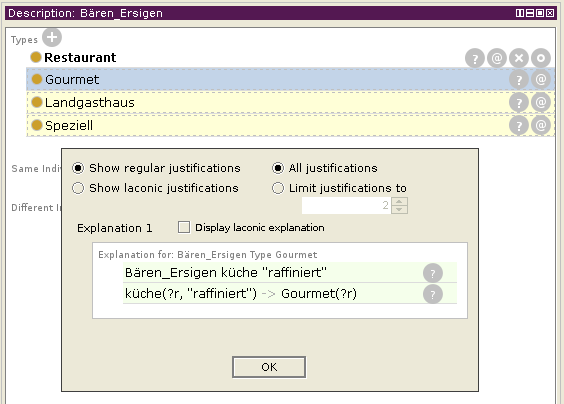
\includegraphics[scale=0.7]{bilder/loesung_regeln.png}
    \caption{Folgerung, dass ein Restaurant ein Gourmetrestaurant ist.\label{fig:loesung:regeln}\protect\footnotemark}
\end{figure}
\footnotetext{Eigene Darstellung mittels Protégé.}

In semantischen Datenbanken gibt es zwei Arten von Eigenschaften. Erstens Objekteigenschaften (ObjectProperties) und zweitens Dateneigenschaften (DataProperties). Objekteigenschaften beschreiben eine Beziehung zwischen zwei Individuen, dadurch werden sie verknüpft. Dateneigenschaften beschreiben eine konkrete Eigenschaft eines Individuums. Sie haften diesem an.

In der erstellten Ontologie wurde die Eigenschaft \textit{Preissegment} als Beziehung, also als ObjectProperty (\textit{hatPreis}) zwischen zwei Individiuen definiert. Daher sind die eigentlichen Preissegmente Individuen der Klasse Preissegment. Jedem Restaurant wird ein Preissegment indirekt zugeteilt. Dies geschieht über die definierte Dateneigenschaft (DataProperty) \textit{Durchschnittspreis}. Liegt der Durchschnittspreis eines Restaurants in einem bestimmten Rahmen, so definieren die Regeln in welchem Preissegment ein Restaurant liegt.


\begin{figure}[H]%[htbp]
    \centering
    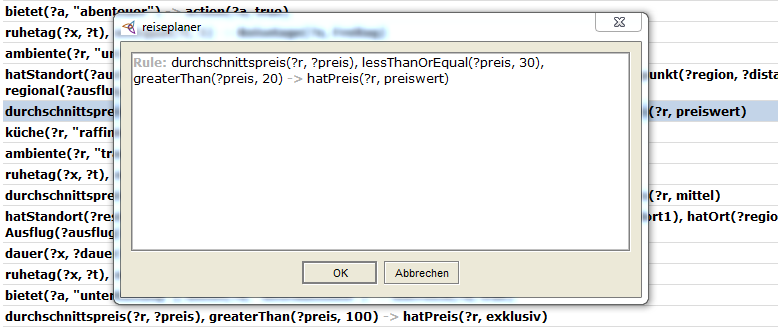
\includegraphics[scale=0.7]{bilder/SWRLBeispiel.png}
    \caption{Regel zur Bestimmung des Preissegmentes ``preiswert''.\label{fig:loesung:regeln_bsp}\protect\footnotemark}
\end{figure}
\footnotetext{Eigene Darstellung mittels Protégé.}

Im Gegensatz zu den Restaurants wurden bei Ausflügen Dateneigenschaften zur Schlussfolgerung verwendet. Die gewünschten Dateneigenschaften kann der Benutzer bei der Suche von Ausflügen anwählen. Beispielsweise kann ein Ausflug, der Wellness bietet, entspannend und romantisch sein.

\begin{figure}[H]%[htbp]
    \begin{minipage}[hbt]{0,49\textwidth}
        \centering
        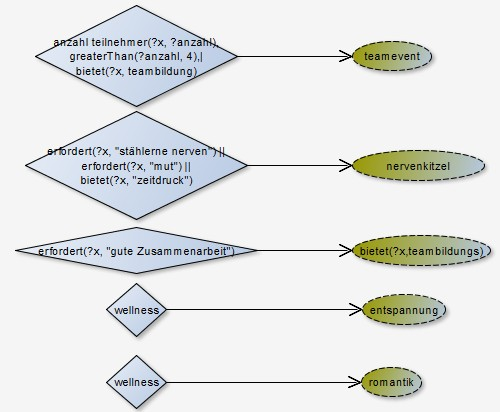
\includegraphics[scale=0.3]{bilder/AufbauAusflug.jpg}
        \caption{Schlussfolgerungen Ausflug.\label{fig:AufbauAusflug}\protect\footnotemark}
    \end{minipage}
    \begin{minipage}[hbt]{0,49\textwidth}
        \centering
        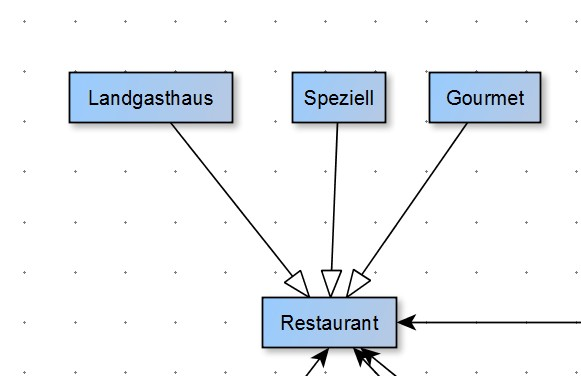
\includegraphics[scale=0.3]{bilder/AufbauRest.jpg}
        \caption{Restaurant-Typen.\label{fig:AufbauRest}\protect\footnotemark[4]}
    \end{minipage}
\end{figure}
\footnotetext{Eigene Darstellung mittels yEd.}

Dadurch, dass beide Suchziele (Restaurant und Ausflug) einer Region und einem Ort zugewiesen sind, mussten die Autoren berücksichtigen, dass der Benutzer für beide Suchziele entscheiden kann, ob er entweder eine von der Region oder von dem Ort abhängige Beschränkung für die Suche festlegen möchte. Die Beziehung zwischen den Regionen oder Orten der Ausflüge bzw. Restaurants wurde mit Hilfe von Objekteigenschaften (ObjectProperties) umgesetzt.\\
Um dem Benutzer die Suche nach Restaurants und Ausflügen in derselben Region bzw.\ demselben Ort zu ermöglichen, haben die Autoren die Objekteigenschaften \textit{gleicherOrt} bzw.\ \textit{gleicheRegion} eingeführt.

Gewisse Ausflugsziele sind nicht ganzjährig erreichbar (der Seilpark Balmberg ist beispielsweise nur von Frühling bis Herbst geöffnet). Durch die Dateneigenschaften (DataProperties) \textit{offenVon} und \textit{offenBis} eines Ausflugzieles kann festgelegt werden, in welchem Zeitraum ein Ausflug möglich ist. Durch entsprechende Regeln wird festgelegt, in welcher Saison ein Ausflugsziel für Besucher geöffnet ist. Hierfür wurde die Klasse \textit{Jahreszeit} mit den entsprechenden Individuen eingeführt.\\
    \begin{figure}[H]%[htbp]
        \begin{minipage}[hbt]{0,49\textwidth}
            \centering
            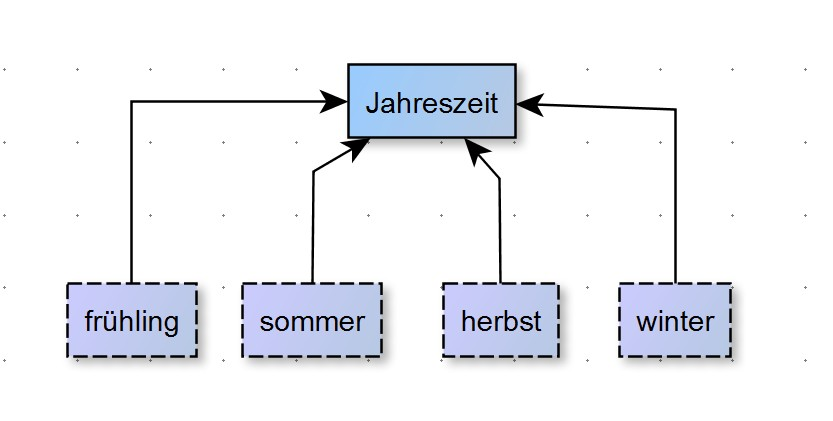
\includegraphics[scale=0.3]{bilder/SaisonKlasse.jpg}
            \caption{Abbildung der Jahreszeiten.\label{fig:SaisonKlasse}\protect\footnotemark}
        \end{minipage}
        \begin{minipage}[hbt]{0,49\textwidth}
            \centering
            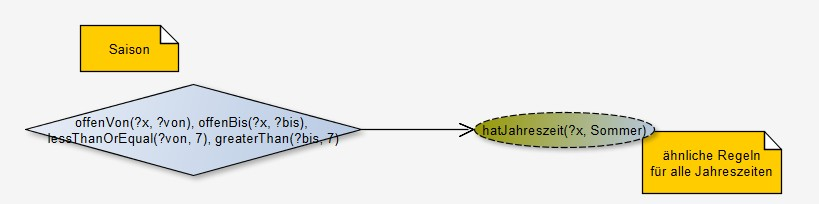
\includegraphics[scale=0.3]{bilder/SaisonRegeln.jpg}
            \caption{Regel zur Bestimmung der Jahreszeiten.\label{fig:SaisonRegeln}\protect\footnotemark[5]}
        \end{minipage}
    \end{figure}


Ein ähnliches Prinzip wurde angewendet, um die Ruhetage eines Ausfluges beziehungsweise eines Restaurants abzubilden. Diese können für jedes Ausflugsziel festgelegt werden. Regeln legen fest, dass der Ausflug an einem bestimmten Tag möglich ist, ausser er sei ein Ruhetag. Diese Festlegung der Ruhetage ist etwas umständlich und nicht sehr intuitiv umgesetzt.

Die Ruhetage bei Ausflugszielen werden durch die Dateneigenschaft \textit{ruhetag} definiert. Dies wird mit einer Zahl von 1 bis 7 (was Montag bis Sonntag entspricht) bezeichnet. Hat ein Ausflug aber keine Ruhetage, so muss diesem dennoch ein Ruhetag zugewiesen werden (eine Zahl die nicht zwischen 1 bis 7 also Montag bis Sonntag liegt). Andernfalls liefern Anfragen keine Ausflüge mehr zurück.

Damit wollen die Autoren eine Einschränkung der Wissensmodellierung mittels Ontologien aufzeigen:\\
Negationen in Regeln sind nicht möglich.\\
Die zur Umsetzung gewählte Methode zeigt dennoch den Vorteil solch einer Modellierung auf. Sie kann beliebig erweitert werden, ohne Notwendigkeit den Programmcode anzupassen.

Ein grösseres Problem bei der Modellierung war die Abbildung von zeitlicher Beschränkung. Ein Benutzer des Reiseplaners soll festlegen können, wieviel Zeit er für eine Reise aufwenden möchte. Im Idealfall würde das System dann alle möglichen Permutationen von Ausflügen berechnen und auflisten. Der Lösung von Planungsproblemen, welche NP-vollständig sind, kann eine ganze Bachelor-Thesis gewidmet werden. Erschwerend kommt hinzu, dass (arithmetische) Berechnungen mittels OWL nur in sehr begrenztem Rahmen möglich sind. Diese Problematik wäre aber mittels Programmlogik zumindest näherungsweise lösbar.

Um die zeitliche Beschränkung von Ausflügen dennoch zu ermöglich, dies aber kein wichtiger Teil der Arbeit sein sollte, haben die Autoren entschieden diese nur in einer einfachen Form abzubilden. Es kann festgelegt werden, wieviel Zeit ein Ausflug in Anspruch nehmen darf. Zur Auswahl stehen die Kriterien halbtags, ganztags und mehrtägig, wobei die mehrtägigen Ausflüge nicht eingearbeitet wurden.\\
In der umgesetzten Version des Reiseplaners werden in der Anfrage immer nur jene Ausflüge ausgegeben, welche der gewünschten Zeiteinheit entsprechen. Um die Dauer eines Ausfluges flexibler zu gestalten haben die Autoren entschieden, dass mehrere Male das Dauer-Attribut gesetzt werden kann. Mit dieser Erweiterung kann ein Ausflug sowohl als halb- als auch als ganztägig deklariert werden.

    \begin{figure}[H]%[htbp]
        \begin{minipage}[hbt]{0,49\textwidth}
            \centering
            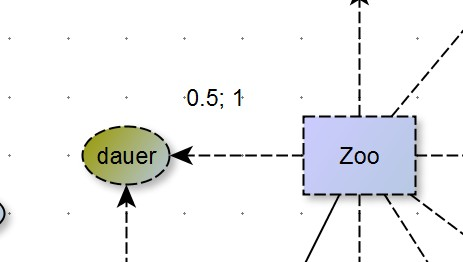
\includegraphics[scale=0.3]{bilder/dauer.jpg}
            \caption*{Dauer eines Ausflugs festlegen.\label{fig:dauer}\protect\footnotemark[5]}
        \end{minipage}
        \begin{minipage}[hbt]{0,49\textwidth}
            \centering
            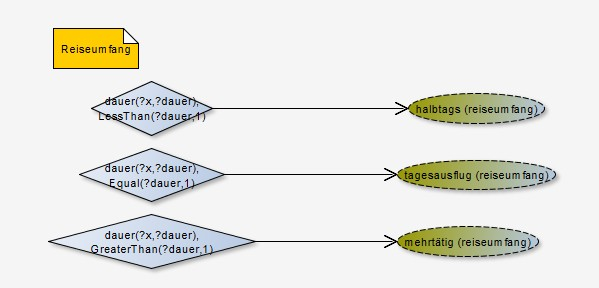
\includegraphics[scale=0.3]{bilder/reiseUmfang.jpg}
            \caption*{Regel zur Bestimmung des Reiseumfangs.\label{fig:reiseumfang}\protect\footnotemark[5]}
        \end{minipage}
    \end{figure}
\footnotetext{Eigene Darstellung mittels yEd.}

\subsection{Mängel in Stardog}
\label{subsec:loesung_modellierung_maengel_stardog}
Bei der Modellierung stiessen die Autoren auf ein für sie zunächst unerklärliches Phänomen: Dem Reasoner von Stardog war es nicht möglich von einer Dateneigenschaften (DataProperty) auf dieselbe Dateneingeschaft zu schliessen. Konkret wollten die Autoren definieren, dass ein Ausflug, der eine Sauna bietet auch Wellness bietet.\\
Auswertung dieser Regel ist aber in Stardog nicht möglich, hingegen wird in Protégé die Schlussfolgerung richtig angezeigt.\\
Nach zahlreichen Recherchen befanden die Autoren, es muss sich bei dieser Einschränkung wohl um einen technischen Fehler in Stardog handeln muss, obwohl beide Werkzeuge den gleichen Reasoner (Pellet) verwenden.\\
Nach dem Fehlermeldung (Bugreporting) in der Diskussionsgruppe von Stardog, wurde den Autoren mitgeteilt, es handele sich wirklich um einen Systemfehler. Um zirkuläre Referenzen im Vorfeld zu verhindern, wurde in Stardog offenbar ein zu strenges Ausschlussverfahren in der Programmlogik verwendet. Der Fehler wurde bereits in einem erfolgten Release korrigiert.\\
Um die gewünschte Folgerung dennoch modellieren zu können, wurde Wellness als Dateneigenschaft vom Typen Boolean definiert und die Regel entsprechend angepasst.

\subsection{Ergebnis}
\label{subsec:loesung_modellierung_ergebnis}
Die Ergebnisse der Modellierung sind:
\begin{itemize}
    \item Ein semantisches Netz
    \item Ein (durch Protégé) generiertes RDF/XML-Dokument
\end{itemize}
Das semantische Netz stellt die Modellierung grafisch dar. Zur besseren Übersicht wurde es in Teilnetze aufgeteilt, wie oben bereits beschrieben. Im RDF/XML-Dokument ist die semantische Datenbank in Form von konkreten Daten abgelegt.

\section{Erstellung von Abfragen}
\label{sec:loesung_sparql}
Für die Modellierung, wie auch für die Datenbankabfragen durch die Benutzeroberfläche (``Suche''), mussten wiederholt Abfragen erstellt werden. Bei einer semantischen Datenbank müssen diese mittels SPARQL gestellt werden. SPARQL ist eine Abfragesprache für Ontologien (Details dazu finden sich im~\hyperref[sec:anhang:tutorial_dokument]{Tutorial} unter Kapitel 10). Durch direkte Integrierung der Abfragen in die erstellte Benutzeroberfläche konnte vermieden werden, dass der Benutzer weder Sprache noch Ontologie kennen muss.

\section{Benutzeroberfläche}
\label{sec:loesung_gui}
Weitere Aufgabe: ``Besondere Bedeutung kommt dabei der Schnittstelle zwischen Mensch und System zu.''~\cite{Aufgabenstellung}

Den Autoren wurde bewusst, dass Abfragen mittels SPARQL sind in keiner Weise benutzerfreundlich. Daher wurde als Benutzerschnittstelle eine Webapplikation zur Reiseplanung entwickelt.\\
Da es für SPARQL keinen Ersatz gibt, musste zur Verständlichkeit ein Assistent entwickelt werden. SPARQL wird weiterhin als Abfragesprache verwendet. 
In der Webapplikation kann der Benutzer mit Hilfe des Assistenten schrittweise Ausflugskriterien wählen. Dadurch ist sichergestellt, dass nur Abfragen gestellt werden können, welche semantisch eine sinnvolle Kombination darstellen.

In einem ersten Schritt kann der Benutzer entscheiden, ob er nur ein Ausflug planen will oder gleichzeitig nach einem Restaurant sucht.\\
Im zweiten Schritt werden dem Benutzer sämtliche Eigenschaften und Beziehungen der zuvor gewählten Ausflugsarten als Auswahl angeboten.\\
Schliesslich erhält der Benutzer eine Liste, die sämtliche den gewählten Kriterien entsprechende Ausflüge enthält. In der Liste sind der Name des Ausflugs, sein Standort und die URL zu seiner Homepage aufgeführt.

Je nach gewählten Kriterien ist es möglich, dass keine Reise gefunden wird. Da nur einige, exemplarische Reisen erfasst wurden, ist bei der Verwendung dieser Webapplikation das Risiko für eine leere Antwort relativ gross.
\begin{figure}[H]
\centering \rotatebox{0}{\scalebox{0.3}[0.3]{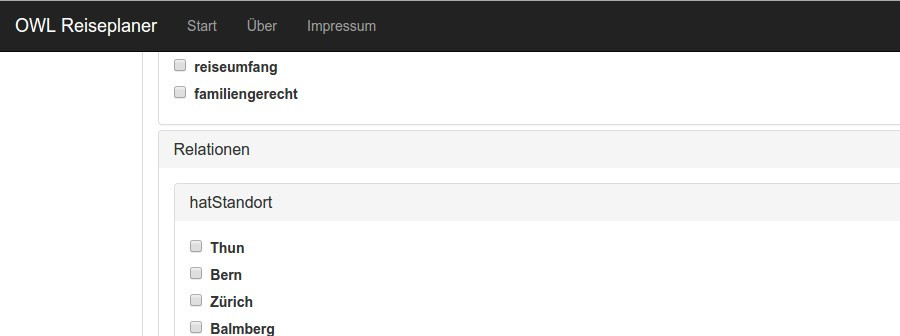
\includegraphics{bilder/reiseplaner_gui.jpg}}}
\caption{Ausschnitt der Benutzeroberfläche. Schritt zwei des Assistenten.\label{fig:gui}\protect\footnotemark}
\end{figure}
\footnotetext{http://elephantsearch.bfh.ch:5820/}
